\documentclass[12pt]{article}

\usepackage{fullpage}
\usepackage{graphicx, rotating, booktabs} 
\usepackage{times} 
\usepackage{natbib} 
\usepackage{indentfirst} 
\usepackage{setspace}
\usepackage{grffile} 
\usepackage{hyperref}
\usepackage{adjustbox}
\setcitestyle{aysep{}}


\singlespace
\title{
\textbf{Appendix: Reassessing the Public Goods Theory of Alliances}
	}
%\author{Joshua Alley\footnote{Graduate Student,
%Department of Political Science, Texas A\&M University.}}

\bibliographystyle{apsr}

\begin{document}

\maketitle 

\doublespace

This appendix contains supporting materials for the tests of Hypothesis 1 and 2. 
The first section includes material for the test of Hypothesis 1. 
The second section describes priors, convergence diagnostics and results from simulated data for the multilevel model I used to test Hypothesis 2. 

%----------------------------------
\section{Other Estimates of Panel Data Interaction}


\subsection{Alternative Estimators}


%Robust regression is appropriate for residuals from the growth variable. 
%Several observations of states during war see gigantic increases in spending--- the largest value is 140, relative to a median of .063. 
%This generates extremely heavy-tailed residuals, so OLS is inefficient. 
%I do not transform spending growth for either test in the paper, but do so here as part of the robustness checks. 
%
%
%Even after applying the inverse hyperbolic sine (IHS) transformation, the residuals deviate strongly from normality as \autoref{fig:res-qq-plot} shows. 
%I use the IHS transformation because it accommodates positive, negative and zero values. 
%\autoref{fig:res-qq-plot} shows the residuals from models 2 and 3 of \autoref{tab:ols-est}, which reports some robustness checks.
%
%\begin{figure}[htbp]
	%\centering
		%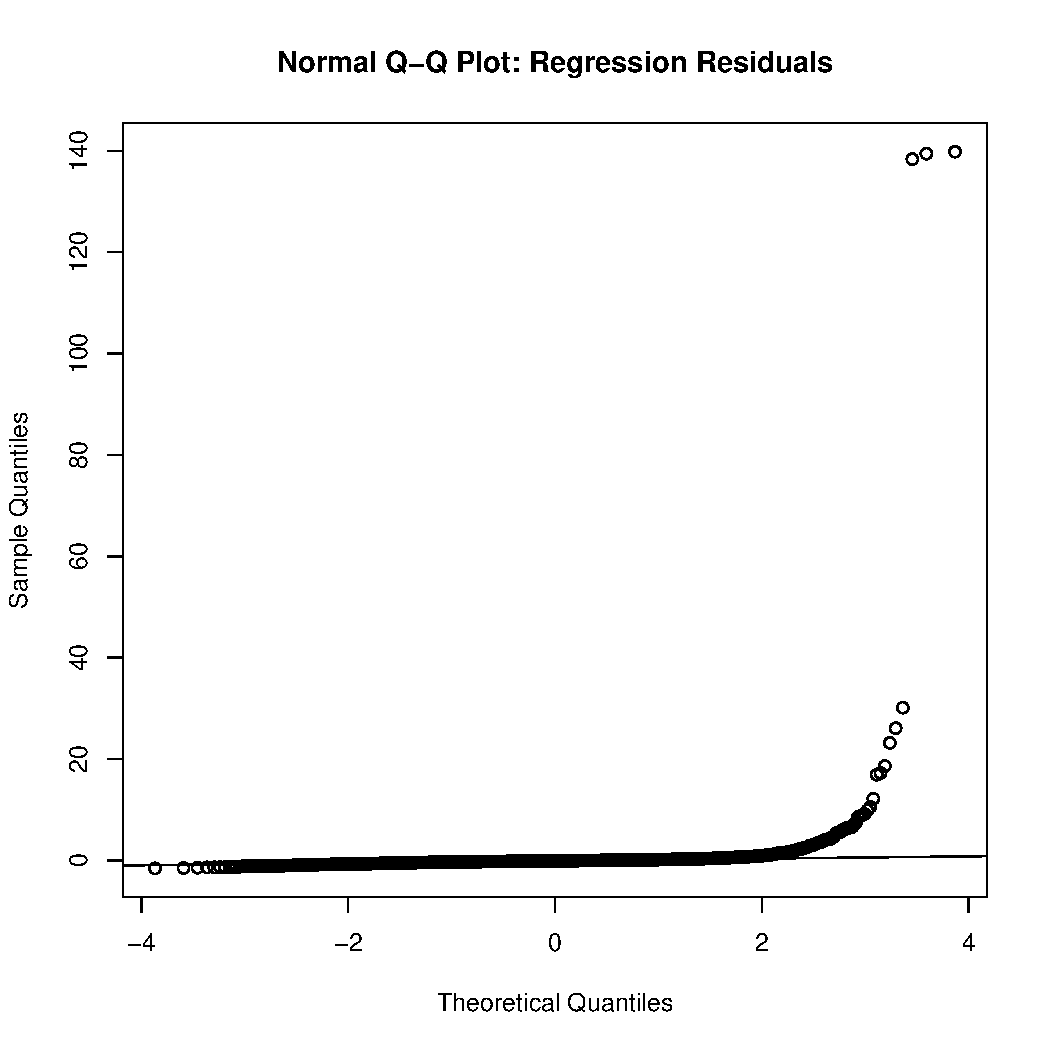
\includegraphics[width=0.95\textwidth]{res-qq-plot.pdf}
	%\caption{Plot of residuals against normal quantiles. Deviations from the straight line are deviations from the normal distribution.}
	%\label{fig:res-qq-plot}
%\end{figure}
%
%
%
%Although OLS is not the best estimator for the spending growth data, it produces similar inferences.
%\autoref{tab:ols-est} summarizes estimates from OLS models with and without transforming growth in spending as well as robust regression with transformed spending. 
%
%\begin{table}[!htbp] \centering 
%\begin{tabular}{@{\extracolsep{5pt}}lccc} 
%\\[-1.8ex]\hline 
%\hline \\[-1.8ex] 
 %& \multicolumn{3}{c}{\textit{Dependent variable:}} \\ 
%\cline{2-4} 
%\\[-1.8ex] & Spending Growth & \multicolumn{2}{c}{IHS(Spending Growth)} \\ 
%\\[-1.8ex] & \textit{OLS} & \textit{OLS} & \textit{Robust Reg.} \\ 
%\\[-1.8ex] & (1) & (2) & (3)\\ 
%\hline \\[-1.8ex] 
 %Change Allied Spending & $-$0.235 & $-$0.099 & $-$0.026 \\ 
  %& (0.648) & (0.087) & (0.047) \\ 
  %& & & \\ 
 %ln(GDP) & $-$0.038$^{**}$ & $-$0.008$^{***}$ & 0.0003 \\ 
  %& (0.017) & (0.002) & (0.001) \\ 
  %& & & \\ 
 %Change Allied Spending $\times$ ln(GDP) & 0.011 & 0.005 & 0.002 \\ 
  %& (0.027) & (0.004) & (0.002) \\ 
  %& & & \\ 	
 %Average Alliance Size & $-$0.003 & $-$0.0001 & 0.0003$^{*}$ \\ 
  %& (0.002) & (0.0003) & (0.0002) \\ 
  %& & & \\ 
 %Average Alliance Democracy & $-$0.001 & $-$0.001 & $-$0.0003 \\ 
  %& (0.008) & (0.001) & (0.001) \\ 
  %& & & \\ 
 %International War & 0.476$^{***}$ & 0.228$^{***}$ & 0.096$^{***}$ \\ 
  %& (0.141) & (0.019) & (0.010) \\ 
  %& & & \\ 
 %Civil War Participant & 0.206$^{**}$ & 0.025$^{*}$ & 0.001 \\ 
  %& (0.104) & (0.014) & (0.008) \\ 
  %& & & \\ 
 %Polity & 0.001 & 0.0001 & $-$0.0001 \\ 
  %& (0.005) & (0.001) & (0.0004) \\ 
  %& & & \\ 
 %External Threat & 0.107 & 0.080$^{***}$ & 0.042$^{***}$ \\ 
  %& (0.152) & (0.021) & (0.011) \\ 
  %& & & \\ 
 %Cold War & 0.032 & 0.034$^{***}$ & 0.047$^{***}$ \\ 
  %& (0.058) & (0.008) & (0.004) \\ 
  %& & & \\ 
 %Constant & 1.074$^{***}$ & 0.259$^{***}$ & 0.026 \\ 
  %& (0.413) & (0.056) & (0.030) \\ 
  %& & & \\ 
%\hline \\[-1.8ex] 
%Observations & 9,139 & 9,139 & 9,139 \\ 
%R$^{2}$ & 0.003 & 0.025 &  \\ 
%Residual Std. Error (df = 9128) & 2.649 & 0.358 & 0.157 \\ 
%\hline 
%\hline \\[-1.8ex] 
%\textit{Note:}  & \multicolumn{3}{r}{$^{*}$p$<$0.1; $^{**}$p$<$0.05; $^{***}$p$<$0.01} \\ 
%\end{tabular} 
%\caption{Robustness checks of conditional relationship between allied spending, GDP and growth in military spending.}
%\label{tab:ols-est}
%\end{table} 
%
%
%The OLS model is a poor fit for the dependent variable. 
%The R$^2$ is miniscule, and the standard error of the residual is much larger than in the robust regression. 
%Transforming the outcome improves the performance of OLS, but leads to similar inferences. 
%Despite the lackluster fit, I present these results to show that OLS generates similar inferences. 


I estimate three different models for the robustness check: OLS models with and without the inverse hyperbolic sine transformation of growth in spending as well as robust regression with transformed spending. 
Rather than interpret the coefficients, I plot the marginal effect of allied spending across the range of GDP for all three models.
\autoref{fig:me-plots} compares these results with the marginal effects plot from the robust regression in the paper. 
Three of the four estimation strategies produce a positive marginal effect, along with broad enough confidence intervals to suggest a conditional relationship with GDP is unlikely.\footnote{The robust regression results are so similar because even after transforming spending growth, the robust estimator heavily down-weights the most unusual observations.} 
OLS without a transformed DV finds no positive impact of changing allied capability on growth in spending, but this result should be taken with great caution due to poor model fit. 
Regardless, none of the results matches the expectation of Hypothesis 1--- a negative effect which increases in state size. 


\begin{figure}[htbp]
	\centering
		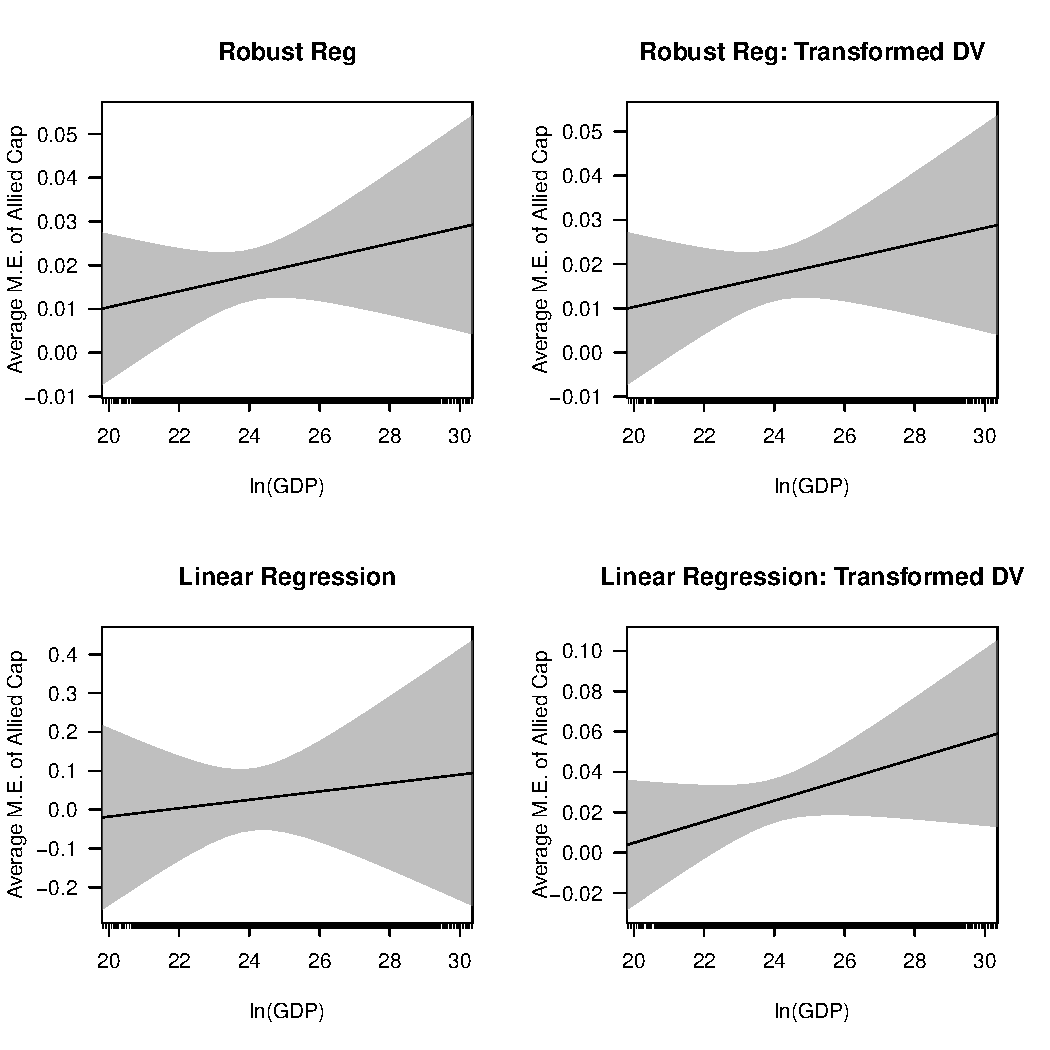
\includegraphics[width=0.95\textwidth]{me-plots.pdf}
	\caption{Comparison of marginal effect of changing allied spending on growth in military spending across the range of GDP. Each plot corresponds to an estimation strategy.}
	\label{fig:me-plots}
\end{figure}



\subsection{Continuous Modifying Variable}


\citet{Hainmuelleretal2019} show linearity assumptions and a lack of support in the range of the modifying variable can generate misleading inferences in interactive models. 
They suggest estimating interactions with binning and kernel estimators to check for non-linearity and adequate support. 
\autoref{fig:inter-bin-abs} plots the results of the binning estimator. 


\begin{figure}
	\centering
		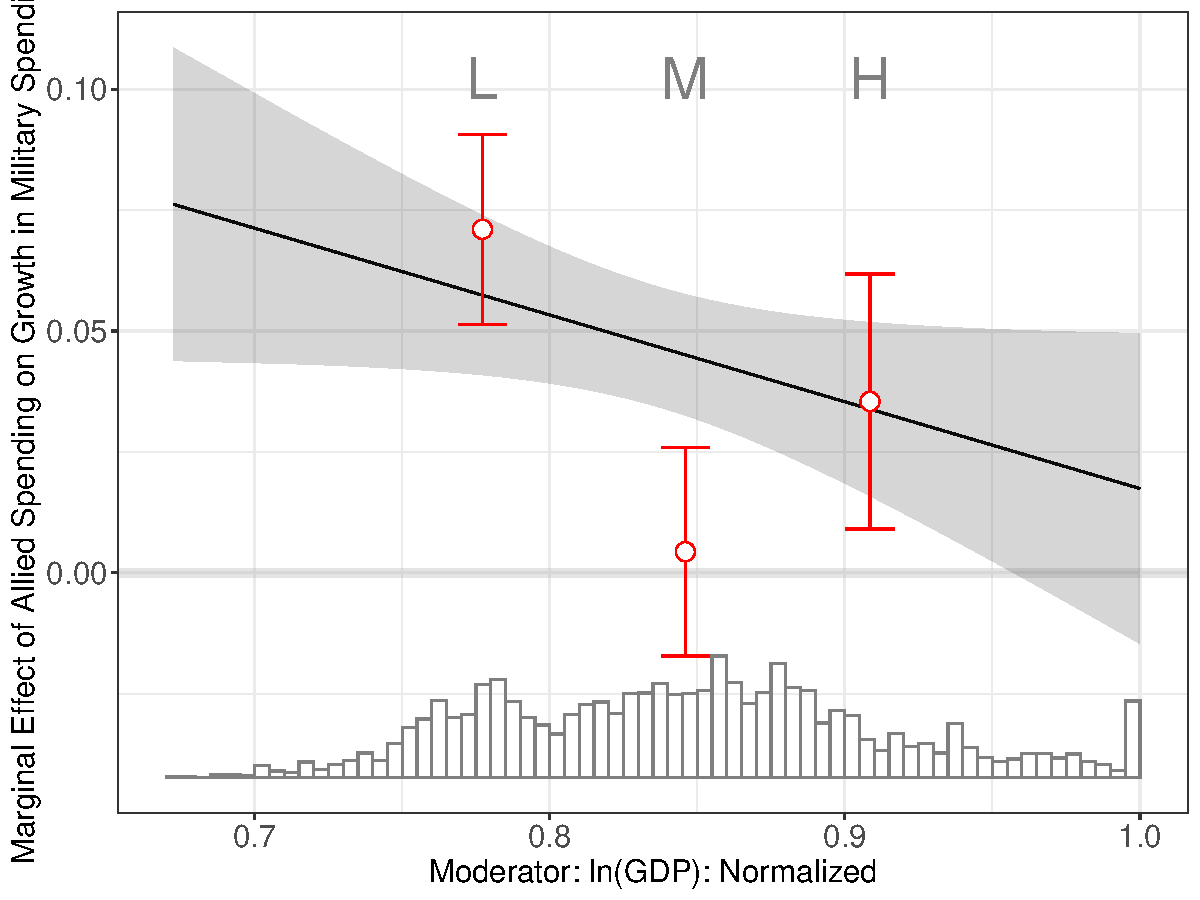
\includegraphics[width=0.65\textwidth]{inter-bin-abs.pdf}
		\caption{Binning estimates of interaction between changes in allied spending and GDP.}
	\label{fig:inter-bin-abs}
\end{figure}


The binning estimator indicates that the linearity assumptions of the robust regression are acceptable. 
There is still no evidence state size modifies the impact of allied spending on growth in military spending, however. 
The marginal effect of allied spending cannot be distinguished from zero across the range of GDP. 


\begin{figure}
	\centering
		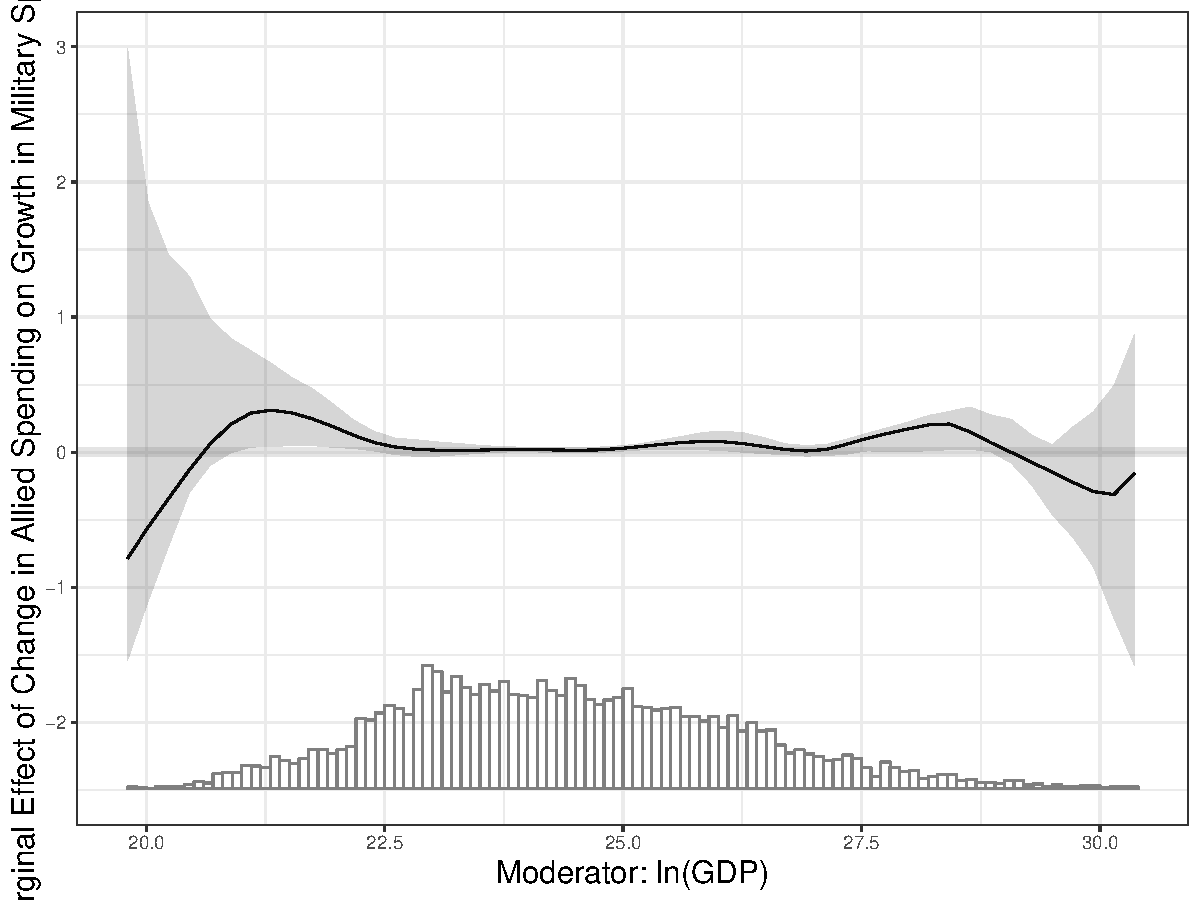
\includegraphics[width=0.65\textwidth]{inter-kernel-abs.pdf}
	\caption{Kernel estimate of interaction between changes in allied spending and GDP.}
	\label{fig:inter-kernel-abs}
\end{figure}


The kernel estimator also generates little evidence of a conditional relationship. 
As \autoref{fig:inter-kernel-abs} demonstrates, the marginal effect of spending is null. 
Both positive and negative point estimates of the marginal effect are indistinguishable from zero. 
Allowing non-linear changes in the marginal effect of allied capability removes the positive marginal effect, it still shows little evidence of a conditional relationship, let alone the expectations of Hypothesis 1. 



\subsection{Robust Regression with Random Effects} 


In the test of Hypothesis 1, the robust regression estimator ignores clustering of observations within groups of states and years. 
\citet{Koller2016} develops a robust regression estimator with random effects, which I fit as a robustness check. 
\autoref{tab:rreg-re-res} summarizes the results. 


\begin{table}[!htbp] \centering 
\begin{tabular}{@{\extracolsep{5pt}} cccc} 
\\[-1.8ex]\hline 
\hline \\[-1.8ex] 
 & Estimate & Std. Error & t value \\ 
\hline \\[-1.8ex] 
Change Allied Spending & $$-$0.015$ & $0.048$ & $$-$0.310$ \\ 
ln(GDP) & $$-$0.002$ & $0.001$ & $$-$1.414$ \\ 
Change Allied Spending $\times$ ln(GDP) & $0.001$ & $0.002$ & $0.661$ \\ 
Avg. Alliance Size & $$-$0.0001$ & $0.0002$ & $$-$0.401$ \\ 
Avg Alliance Democracy & $$-$0.001$ & $0.001$ & $$-$1.354$ \\ 
International War & $0.096$ & $0.011$ & $8.889$ \\ 
Civil War Participant & $0.010$ & $0.008$ & $1.299$ \\ 
Polity & $0.0002$ & $0.0004$ & $0.657$ \\ 
External Threat & $0.016$ & $0.013$ & $1.217$ \\ 
Cold War & $0.060$ & $0.011$ & $5.242$ \\ 
Constant & $0.075$ & $0.031$ & $2.436$ \\ 
\hline \\[-1.8ex] 
\end{tabular} 
\caption{Results from Robust Regression with State and Year random effects.} 
\label{tab:rreg-re-res} 
\end{table} 


Robust regression with random effects produces similar inferences about the presence of a conditional relationship between GDP and changing allied capability. 
The sign, magnitude and statistical significance of all the coefficients are similar to results from other estimators. 
Therefore, while it is difficult to use \textsf{R} output from Koller's robust regression estimator to plot the interaction, results from this estimator should mirror the above plots. 
Accounting for clustering of observations does little to change my inferences about Hypothesis 1. 


\section{Multilevel Model}

This section describes the priors on the multilevel model, convergence diagnostics for the Hamiltonian Monte Carlo, and results from running the same model on a sample of only states with at least one alliance. 

\subsection{Priors} 

All priors are specified to be weakly informative relative to the scale of the data \citep{Gelmanetal2017}. 
I summarize the prior distributions for each set of parameters in \autoref{tab:priors}. 
$p(\nu)$ is a well-behaved prior for the degrees of freedom in a t-distribution \citep{JuarezSteele2010}. 
Given that median growth in military expenditures is 0.06, the priors are quite diffuse. 


\begin{table} % Create a table of priors.
\begin{center}
\begin{tabular}{c} 
$ p(\alpha) \sim N(0, 1)$  \\
$ p(\sigma) \sim \mbox{half-}N(0, 1) $ \\
$ p(\alpha^{yr}) \sim N(0, \sigma^{yr}) $ \\ 
$ p(\sigma^{yr}) \sim N(0, 1) $ \\
$ p(\alpha^{st}) \sim N(0, \sigma^{st}) $ \\ 
$ p(\sigma^{st}) \sim \mbox{half-}N(0, 1) $ \\ 
$ p(\gamma) \sim N(\theta, \sigma^{all}) $ \\ 
$ p(\theta) \sim N(0, .5) $ \\
$ p(\sigma^{all}) \sim \mbox{half-}N(0, 1) $ \\
$ p(\beta) \sim N(0, 1) $ \\
$ p(\nu) \sim gamma(2, 0.1)$ 
\end{tabular} 
\caption{Summary of Priors in Multilevel Model} 
\label{tab:priors}
\end{center} 
\end{table} 


To facilitate estimation, I use a non-centered parameterization for the state and year varying intercepts, as well as the $\gamma$ parameters \citep{BetancourtGirolani2015}. 
A non-centered parameterization decouples the mean and variance to express an equivalent prior, which makes sampling easier. 
I also employ a sparse matrix representation of the alliance membership matrix $\textbf{Z}$ to speed up estimation. 


\subsection{Convergence} 


There were no divergent iterations in sampling. 
However, there are other threats to inference from the posterior samples. 
Given heavy tails in military spending growth, STAN might have struggled to explore the posterior distribution. 


Energy plots can diagnose this problem. 
\autoref{fig:energy-plot} plots the marginal energy distribution and the first differenced distribution. 
If the two histograms do not overlap, sampling was impeded by heavy tails. 
The substantial overlap in the distributions for all four chains in \autoref{fig:energy-plot} indicates this was not a problem. 


\begin{figure}
	\centering
		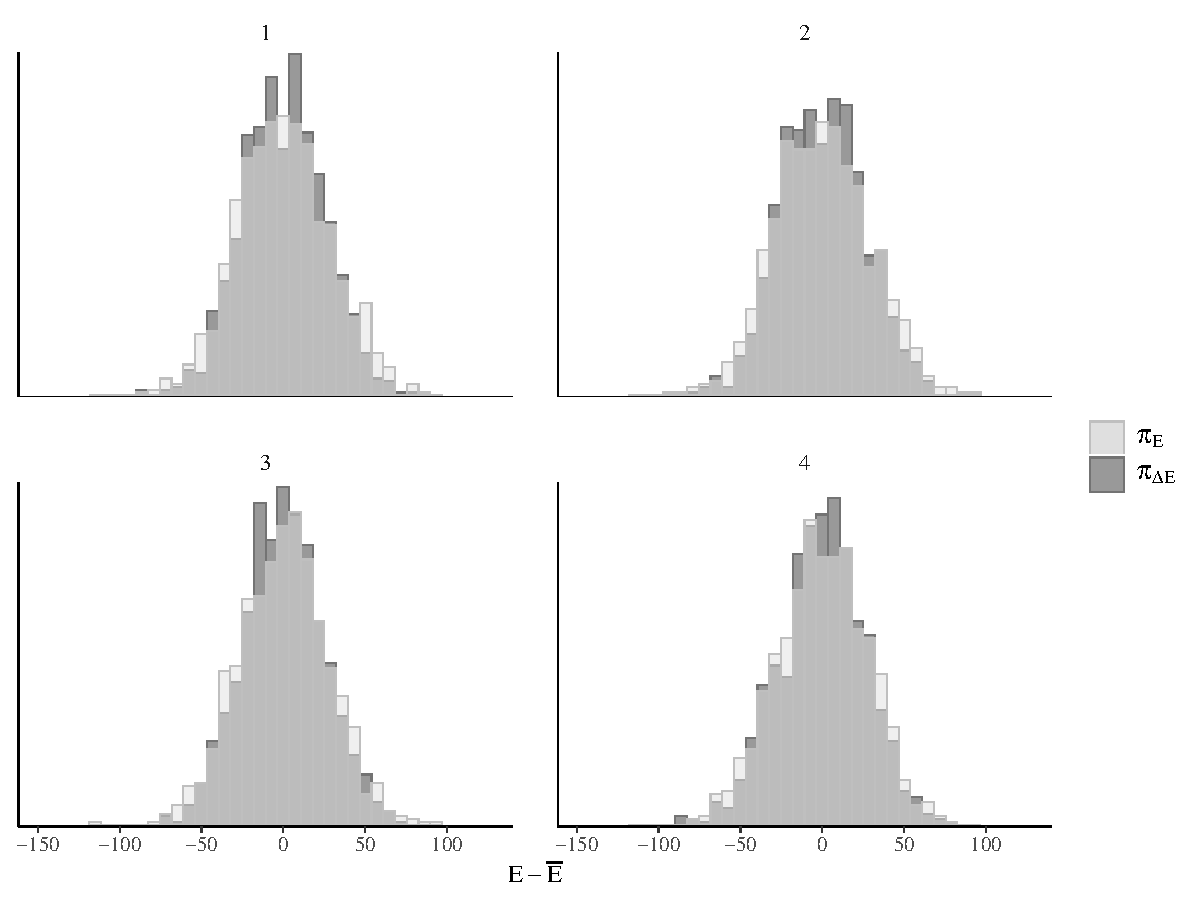
\includegraphics[width=0.55\textwidth]{energy-plot.pdf}
	\caption{Energy plot of multilevel model results. Greater overlap in the two histograms indicates adequate exploration of the posterior distribution. }
	\label{fig:energy-plot}
\end{figure}


The split $\hat{R}$ statistic is another way to assess convergence. 
$\hat{R}$ compares the behavior of each chain by measuring the ratio of the average variance of draws within each chain to the variance of the pooled draws across chains. 
When $\hat{R}$ is close to 1, all the chains have similar variance, and are therefore in equilibrium. 


The standard heuristic is that an $\hat{R}$ greater than 1.1 is problematic. 
\autoref{fig:rhat-plot} plots the $\hat{R}$ statistic for every parameter in the model. 
No parameters generate concern, even at a more conservative threshold of 1.05. 


\begin{figure}[htbp]
	\centering
		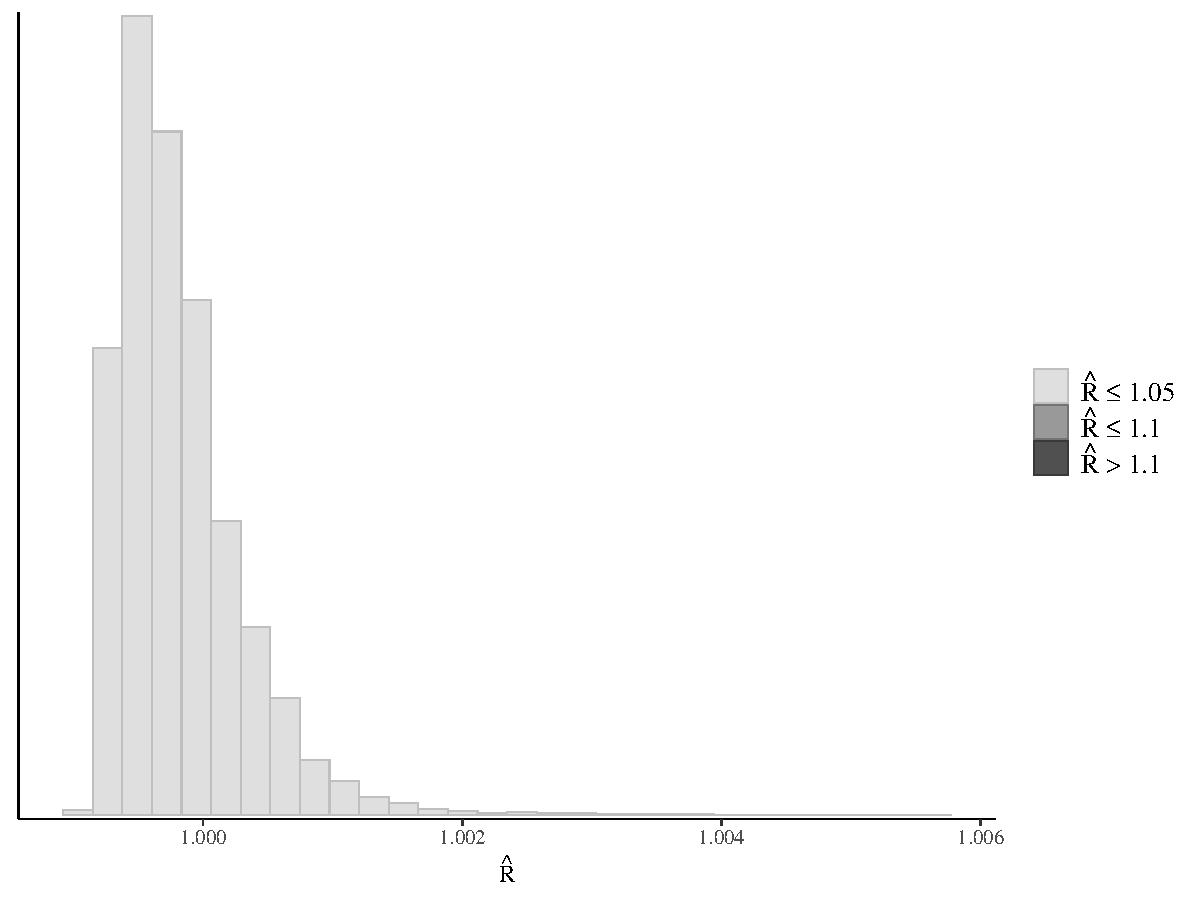
\includegraphics[width=0.55\textwidth]{rhat-plot.pdf}
	\caption{Histogram of split $\hat{R}$ statistic for all parameters in the multilevel model.}
	\label{fig:rhat-plot}
\end{figure}


\subsubsection{Inferences from Simulated Data}


To assess if the model gives reasonable answers, I simulated data and associated parameters, then re-estimated the model on the simulated data.
The model is a good fit if the credible intervals contain the known parameter values for the simulated data. 
This process checks whether the model can recover parameters from a known data-generating process that matches the model. 


I simulate a hypothetical dataset with 5000 observations of 50 states observed over 200 years. 
There are 200 alliances in this data, and 2 state-level control variables. 
The hypothetical outcome is drawn from a Cauchy distribution with mean 0 and a scale of .25, which is more heavy-tailed than even my observed growth data. 


I then simulate 2,000 draws of the outcome using the generated quantities block in STAN. 
The next step is selecting one of those draws of the outcome--- which includes the value of the outcome for each observation and the associated parameter values. 
I select the 12th draw from the posterior and check whether after estimating the model on these data, the credible intervals include zero. 


I focus on inferences about the $\gamma$, $\theta$ and $\sigma_{all}$ parameters, because these are essential to testing the public goods argument. 
As \autoref{fig:theta-sim-res} and \autoref{fig:sall-sim-res} show, the posteriors accurately capture the known values of the hyper-parameters $\theta$ and $\sigma_{all}$. 
In these figures, the true parameter value is marked with a thick black line, while the light gray shaded area shows the 90\% credible interval. 


\begin{figure}[htbp]
	\centering
		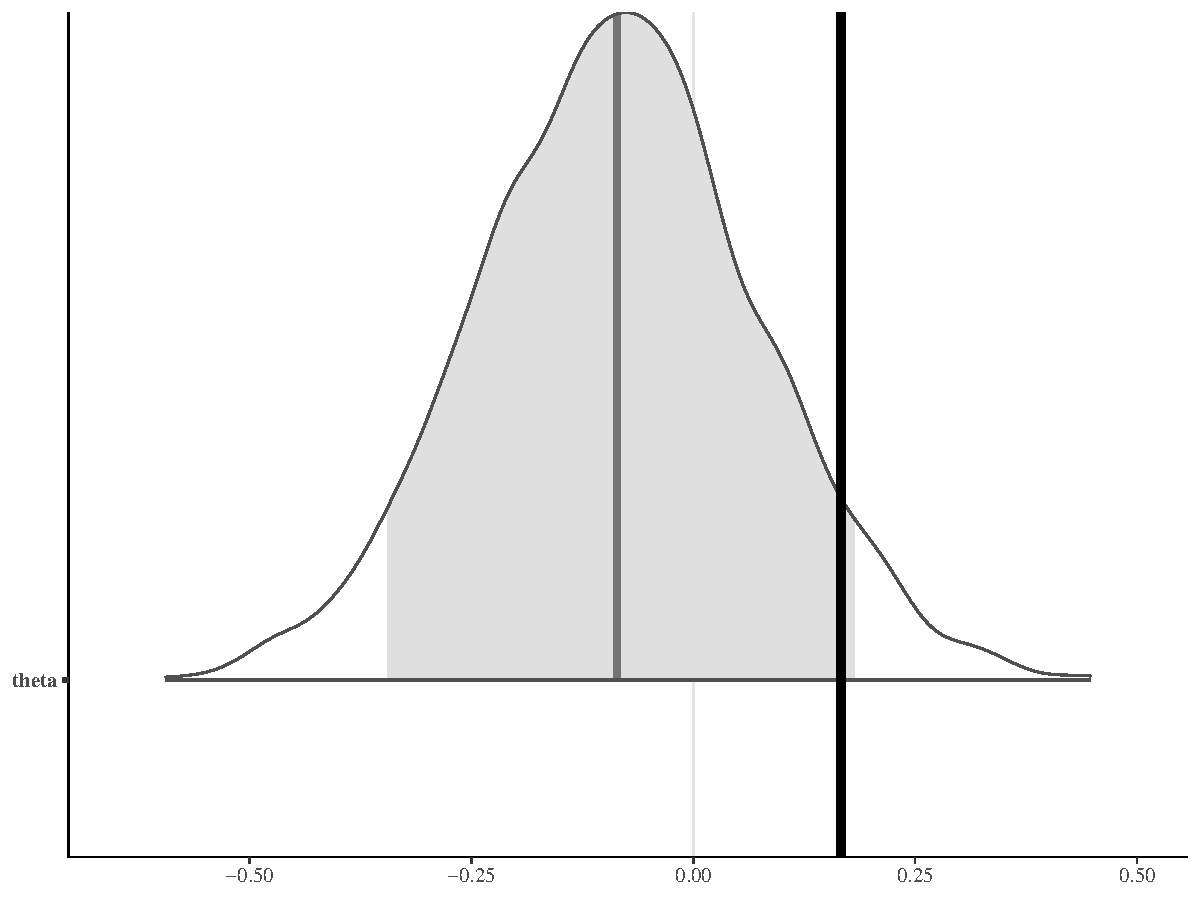
\includegraphics[width=0.65\textwidth]{theta-sim-res.pdf}
	\caption{Posterior estimates and known parameter value for the alliance hyperparameter $\theta$. The dark gray bar marks the posterior mean, while the shaded area captures the 90\% credible interval. The black line marks the known, ``true'' $\theta$ value, which falls within the 90\% interval.}
	\label{fig:theta-sim-res}
\end{figure}


\begin{figure}[htbp]
	\centering
		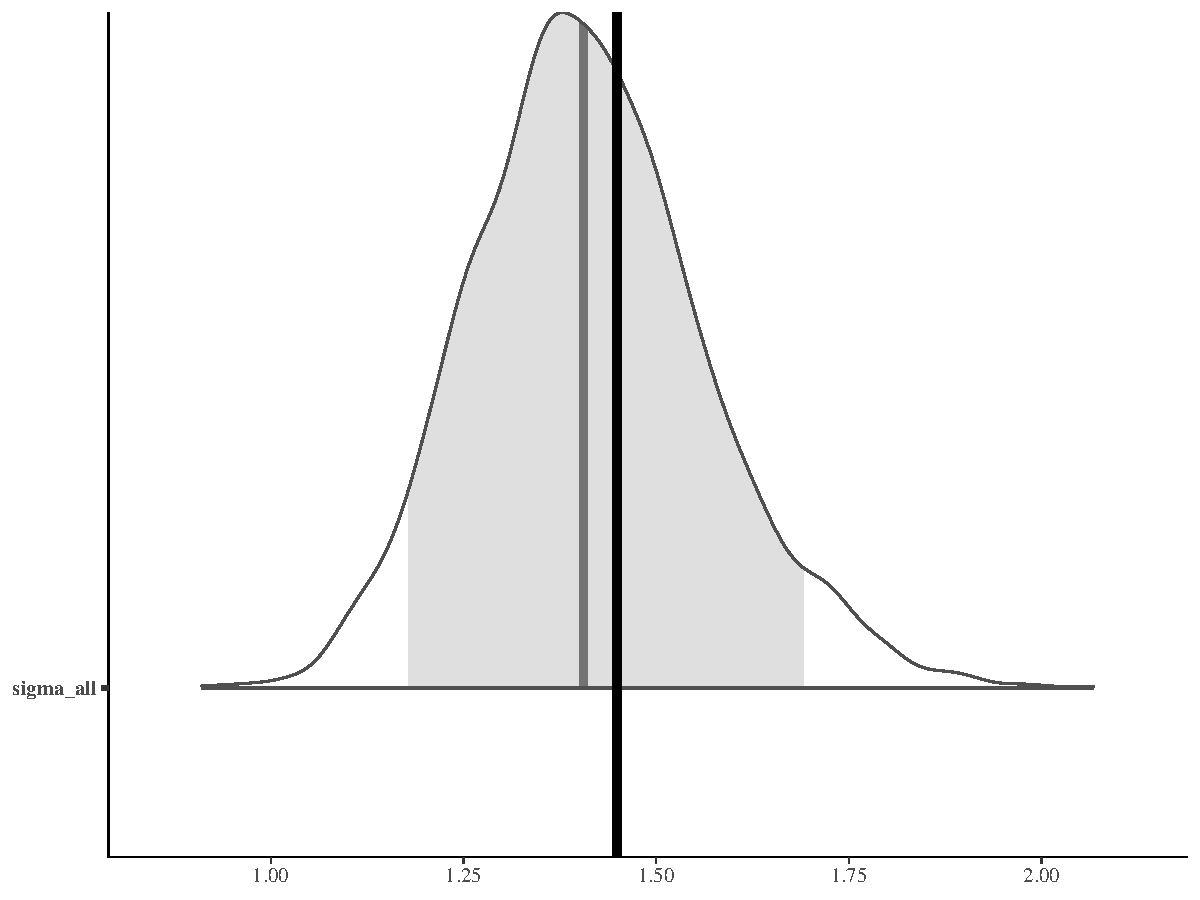
\includegraphics[width=0.65\textwidth]{sall-sim-res.pdf}
	\caption{Posterior estimates and known parameter value for the alliance hyperparameter $\sigma_{all}$. The dark gray bar marks the posterior mean, while the shaded area captures the 90\% credible interval. The black line marks the known, ``true'' $\sigma_{all}$ value, which falls within the 90\% interval.}
	\label{fig:sall-sim-res}
\end{figure}


Because graphical presentation of the 200 $\gamma$ parameters is more difficult, I calculated whether the credible interval contained the known parameter. 
184 of the 200 intervals include the ``true'' $\gamma$ value, which is a 92\% success rate. 
Given the number of parameters and potential simulation variance, such accuracy is tolerable. 
Simulating data and recovering known parameters shows that the model estimates are reasonable approximations of the data-generating process. 
 



%\subsection{Alternative Sample} 
%
%
%It is possible that estimating a model on the full sample of states makes misleading comparisons by including states with no alliances.
%This adds many zeros to the membership matrix. 
%To check whether inferences are sensitive to including states with no alliance participation, I re-fit the multilevel model on a sample of only states with at least one alliance. 
%This reduced the sample size from 9,961 observations to 5,222, but the results are relatively unchanged. 
%
%
%All 285 treaties have a negative mean $\gamma$ estimate, and none have a 90\% credible interval that excludes zero.
%The overall mean $\theta$ is more negative in this sample and the $\gamma$ estimates remain tightly clustered around that mean. 
%Thus as \autoref{fig:sample-comp-gamma} shows, the distribution of the association between treaty contribution and spending across alliances is more negative in the alliance members sample. 
%This figure overlays the distribution of the mean $\gamma$ parameters in each sample. 
%
%
%\begin{figure}
	%\centering
		%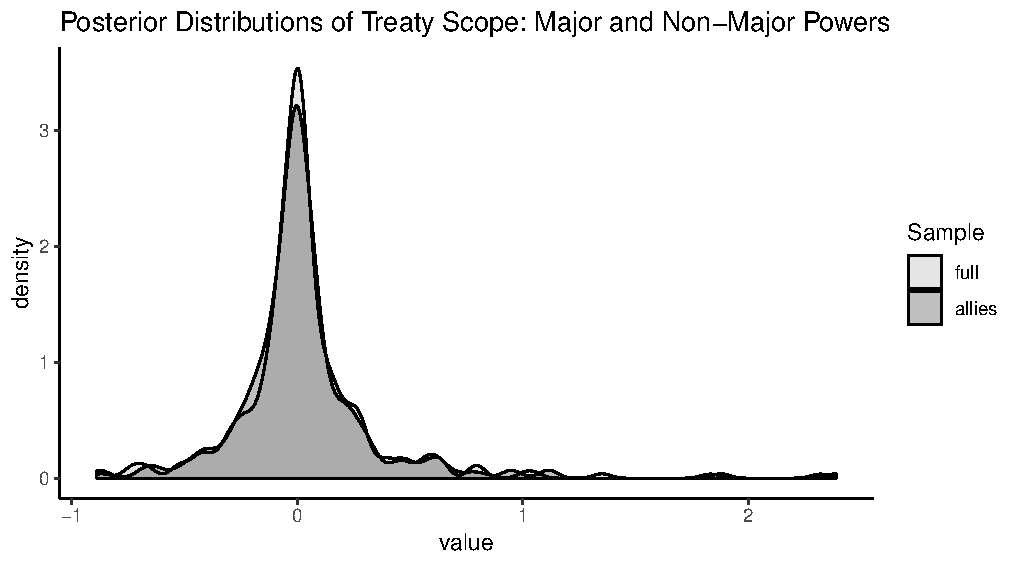
\includegraphics[width=0.95\textwidth]{sample-comp-gamma.pdf}
	%\caption{Comparison of the distribution of posterior mean $\gamma$ parameters in full sample and a sample of only alliance participants. The darker gray distribution is the mean of the $\gamma$ parameters in the sample of alliance members. The impact of treaty contribution on growth in military spending is more negative in the alliance-members only sample.}
	%\label{fig:sample-comp-gamma}
%\end{figure}
%
%
%Therefore, inferences about the impact of treaty contribution on growth in military spending are unchanged if the sample is restricted only to alliance members. 
%Increasing a state's share of total allied GDP leads to a more negative effect on treaty spending in expectation. 
%I am still unable to identify any reliably positive $\gamma$ parameters, which contradicts Olson and Zeckhauser's exploitation hypothesis. 








\singlespace


\bibliography{../../../MasterBibliography} 





\end{document}
